\documentclass[border=8pt]{standalone}
\usepackage{fontspec}
\setmainfont{TeX Gyre Heros}[Ligatures=TeXOff]
\XeTeXgenerateactualtext=1
\setsansfont{TeX Gyre Heros}
\usepackage{tikz}
\usetikzlibrary{arrows.meta,positioning,shapes.geometric,shapes.misc,shapes.symbols,fit,backgrounds,calc,chains}
\definecolor{ink}{HTML}{111827}
\definecolor{band}{HTML}{F3F4F6}
\definecolor{band2}{HTML}{E5E7EB}
\definecolor{accent}{HTML}{1D4ED8}
\definecolor{accentlight}{HTML}{DBEAFE}
\definecolor{warn}{HTML}{B91C1C}
\definecolor{warnlight}{HTML}{FEE2E2}
\definecolor{ok}{HTML}{047857}
\definecolor{oklight}{HTML}{D1FAE5}
\tikzset{
  >={Stealth[length=2.6mm]},
  box/.style={draw=ink, line width=0.6pt, rounded corners=9pt, fill=white, align=center,
              inner sep=4pt, font=\small},
  pill/.style={box, rounded corners=13pt},
  key/.style={box, fill=accentlight, draw=accent, line width=0.9pt},
  soft/.style={box, fill=band},
  dec/.style={draw=ink, line width=0.6pt, diamond, aspect=2.2, align=center, inner sep=1.5pt,
              font=\footnotesize, fill=white},
  arr/.style={->, draw=ink, line width=0.6pt},
  darr/.style={->, draw=ink, line width=0.6pt, dashed},
  lbl/.style={font=\footnotesize, fill=white, inner sep=1.5pt},
  layer/.style={draw=band2, fill=band, rounded corners=6pt},
  title/.style={font=\bfseries\small, align=left, anchor=west},
}
\begin{document}
\sffamily\hyphenpenalty=10000\exhyphenpenalty=10000

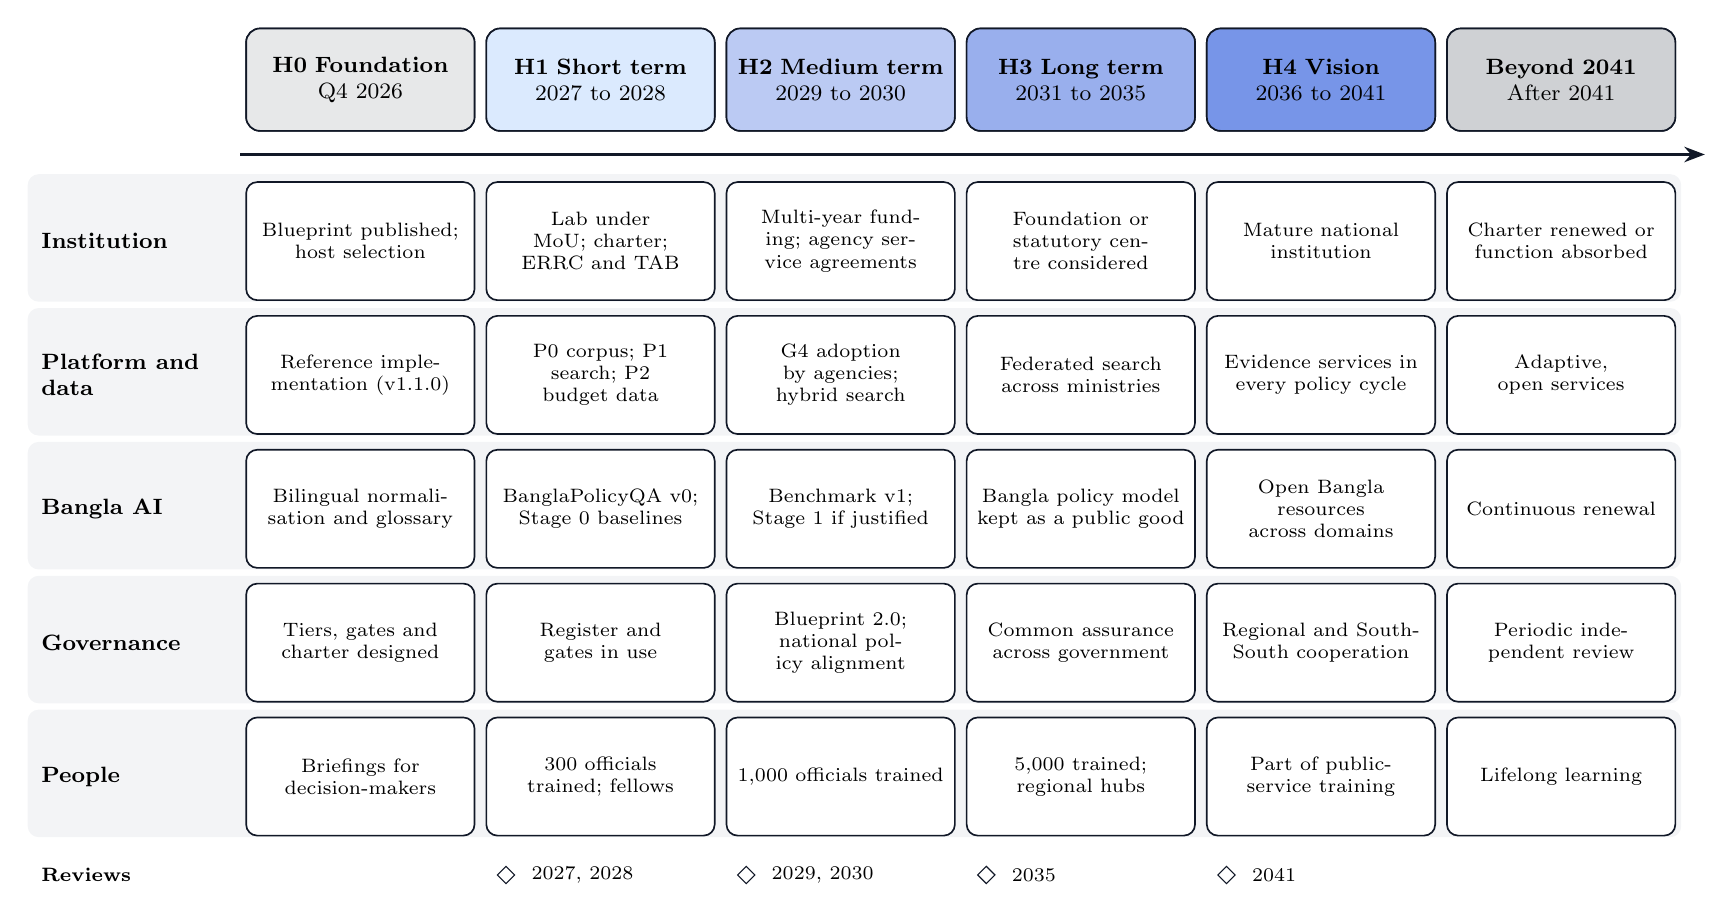
\begin{tikzpicture}
\def\L{27mm}\def\C{30.5mm}\def\R{17mm}
\tikzset{hd/.style={box, rounded corners=5pt, minimum width=\C-1.5mm, minimum height=13mm, text width=\C-3mm, font=\footnotesize, inner sep=2pt},
         cell/.style={box, rounded corners=4pt, minimum width=\C-1.5mm, minimum height=\R-2mm, text width=\C-4mm, font=\scriptsize, inner sep=1.5pt},
         ln/.style={font=\footnotesize\bfseries, text width=\L-3mm, align=left, anchor=west}}
\foreach \c/\col in {0/ink!10,1/accentlight,2/accent!30,3/accent!45,4/accent!60,5/ink!20} {
  \node[hd, fill=\col] (h\c) at (\L+\c*\C+0.5*\C, 0) {};
}
\node[hd, fill=ink!10] at (h0) {\textbf{H0 Foundation}\\Q4 2026}; \node[hd, fill=accentlight] at (h1) {\textbf{H1 Short term}\\2027 to 2028};
\node[hd, fill=accent!30] at (h2) {\textbf{H2 Medium term}\\2029 to 2030}; \node[hd, fill=accent!45] at (h3) {\textbf{H3 Long term}\\2031 to 2035};
\node[hd, fill=accent!60] at (h4) {\textbf{H4 Vision}\\2036 to 2041}; \node[hd, fill=ink!20] at (h5) {\textbf{Beyond 2041}\\After 2041};
\draw[arr, line width=1.2pt] (\L,-9.5mm) -- (\L+6*\C+3mm,-9.5mm);
\newcommand{\lane}[8]{%
  \fill[band, rounded corners=4pt] (0,-12mm-#1*\R) rectangle (\L+6*\C,-12mm-#1*\R-\R+0.8mm);
  \node[ln] at (0.5mm,-12mm-#1*\R-0.5*\R) {#2};
  \node[cell] at (\L+0.5*\C,-12mm-#1*\R-0.5*\R) {#3};
  \node[cell] at (\L+1.5*\C,-12mm-#1*\R-0.5*\R) {#4};
  \node[cell] at (\L+2.5*\C,-12mm-#1*\R-0.5*\R) {#5};
  \node[cell] at (\L+3.5*\C,-12mm-#1*\R-0.5*\R) {#6};
  \node[cell] at (\L+4.5*\C,-12mm-#1*\R-0.5*\R) {#7};
  \node[cell] at (\L+5.5*\C,-12mm-#1*\R-0.5*\R) {#8};}
\lane{0}{Institution}{Blueprint published; host selection}{Lab under MoU; charter; ERRC and TAB}{Multi-year funding; agency service agreements}{Foundation or statutory centre considered}{Mature national institution}{Charter renewed or function absorbed}
\lane{1}{Platform and data}{Reference implementation (v1.1.0)}{P0 corpus; P1 search; P2 budget data}{G4 adoption by agencies; hybrid search}{Federated search across ministries}{Evidence services in every policy cycle}{Adaptive, open services}
\lane{2}{Bangla AI}{Bilingual normalisation and glossary}{BanglaPolicyQA v0; Stage 0 baselines}{Benchmark v1; Stage 1 if justified}{Bangla policy model kept as a public good}{Open Bangla resources across domains}{Continuous renewal}
\lane{3}{Governance}{Tiers, gates and charter designed}{Register and gates in use}{Blueprint 2.0; national policy alignment}{Common assurance across government}{Regional and South-South cooperation}{Periodic independent review}
\lane{4}{People}{Briefings for decision-makers}{300 officials trained; fellows}{1,000 officials trained}{5,000 trained; regional hubs}{Part of public-service training}{Lifelong learning}
\foreach \c/\t in {1/{2027, 2028},2/{2029, 2030},3/{2035},4/{2041}} {
  \node[draw=ink, fill=white, diamond, inner sep=1.6pt] at (\L+\c*\C+0.5*\C-12mm,-12mm-5*\R-4mm) {};
  \node[font=\scriptsize, anchor=west] at (\L+\c*\C+0.5*\C-10mm,-12mm-5*\R-4mm) {\t};
}
\node[font=\scriptsize\bfseries, anchor=west] at (0.5mm,-12mm-5*\R-4mm) {Reviews};
\end{tikzpicture}
\end{document}
